\documentclass[conference,10pt]{IEEEtran}

\usepackage{cite}
\usepackage{amsmath,amssymb}
\usepackage{graphicx}
\usepackage{tabularx}
\usepackage{placeins}
\usepackage[hidelinks]{hyperref}

% Keep figure descriptions in the source for future accessible output.
\newcommand{\Description}[1]{}
\setlength{\emergencystretch}{1em}


\title{Thermal-Aware NoC Reconfiguration for MoE Inference in 3D DRAM-Stacked Systems}
\author{Anonymous Author(s)}

\begin{document}


\maketitle

\begin{abstract}
Three-dimensional DRAM stacking provides high memory bandwidth for Mixture-of-Experts (MoE) inference, but efficiently utilizing distributed compute and memory resources remains challenging. Input-dependent expert activation and concentrated memory accesses produce uneven communication demands that change across execution stages, causing contention on shared network paths. Thermal coupling between stacked logic and memory dies further limits sustained performance. Coarse-grained bandwidth configurations offer limited flexibility in allocating connectivity to changing heavy flows. We propose traffic- and thermal-aware NoC reconfiguration for MoE inference in 3D DRAM-stacked systems. Interconnected configurable switches establish dedicated paths for selected high-volume and long-range flows, reducing competition for router forwarding resources. A prediction mechanism estimates communication demand from expert activation and memory access behavior. Based on this demand, a configuration algorithm selects compatible switch connections to maximize the traffic accommodated by dedicated paths under physical port and path-conflict constraints. Coupled thermal prediction further guides task placement and regional voltage--frequency adjustment to alleviate cross-tier hotspots while limiting execution-time overhead.
\end{abstract}

\begin{IEEEkeywords}
hybrid bonding, 3D integration, mixture-of-experts, network-on-chip,
reconfigurable interconnect, memory-bank contention, thermal management
\end{IEEEkeywords}
\raggedbottom

\section{Introduction}
\label{sec:introduction}

The rapid growth of AI models is increasing demands for compute throughput,
memory capacity, and data-movement bandwidth, motivating three-dimensional (3D)
integration of heterogeneous compute and memory resources. Commercial systems
such as AMD's hybrid-bonded 3D V-Cache demonstrate the maturity of this approach,
while Helios applies hybrid-bonded 3D DRAM to near-memory processing for
large language model (LLM) serving~\cite{wuu2022vcache,li2026helios}.

Deploying LLM inference on such 3D systems exposes three interrelated
challenges. First, uneven accesses to model parameters and KV-cache data cause
DRAM-bank conflicts,causing an increase in the delay of memory access time. Second, bursty and spatially skewed communication causes
network-on-chip (NoC) contention when messages compete for the same links or
router outputs. The busy resources can change between mixture-of-experts
(MoE) model layers and communication phases, whereas a small set of
predefined topologies offers limited ways to adapt local connections. Third, spatially aligned activity in the stacked Logic and DRAM tiers
creates vertically coupled thermal hotspots, increasing peak temperature and
the risk of thermal throttling.

Prior work addresses these challenges through expert placement, interconnect
configuration, and thermal management. HiBand
combines bank-local HB-DRAM, hierarchical data movement, and a small set of
reconfigurable NoC modes~\cite{wang2026hiband}; Sem-MoE co-schedules expert
placement and token routing to increase device-local expert activations
~\cite{li2026semantic}; and AMBER combines offline thermal-aware mapping with
online subtask interleaving and DVFS~\cite{lin2026amber}. 


Our experiments identify three remaining bottlenecks in memory access,
on-chip communication, and thermal management. Concurrent Qwen3 requests
contend for shared DRAM banks, delaying memory accesses. During Qwen3
prefill, uneven traffic creates queues along shared network paths.
In the thermal study, AMBER-style management reduces throughput relative
to the reference without thermal control, while hotspots remain aligned
across the logic and DRAM tiers. These observations motivate examining how
memory accesses and NPU-to-NPU messages compete for shared resources and
how activity in the stacked tiers contributes to cross-tier hotspots.

To address the above challenges, we distribute concurrent memory accesses
across DRAM banks and configure dedicated NoC paths for selected flows
in each MoE communication phase to reduce queueing at congested links
and router outputs. We also use coupled logic--DRAM thermal predictions
to guide task placement and regional voltage and frequency adjustments,
while accounting for data-copy and activation-transfer costs.

The contributions of the paper are as follows:
\begin{enumerate}
  \item We identify phase-dependent NoC congestion in MoE inference on
  3D DRAM-stacked systems. Input-dependent expert activation and concentrated
  memory accesses create uneven communication demand, while coarse-grained NoC
  configurations limit the ability to redirect traffic away from congested
  links and router outputs. We also observe persistent cross-tier hotspots
  under thermal management.

  \item We propose a framework that jointly optimizes NoC reconfiguration,
  DRAM-bank placement, and thermal-aware execution. It configures dedicated
  paths for predicted heavy flows under physical port and path-conflict
  constraints, distributes concurrent accesses across DRAM banks, and uses
  coupled logic--DRAM thermal predictions to guide task placement and regional
  DVFS. These mechanisms aim to reduce network queueing and bank contention
  while mitigating cross-tier hotspots.

  \item Across the evaluated MoE workloads, the proposed framework reduces
  mean NoC queueing latency by xxx\% relative to the baseline. The estimated
  end-to-end inference latency decreases by xxx\%, and the peak stack
  temperature decreases by xxx~$^\circ$C under matched thermal conditions.
\end{enumerate}

\setlength{\textfloatsep}{12pt}
\setlength{\floatsep}{10pt}

\section{Motivation}
\label{sec:motivation}

\subsection{Target System and Workloads}
\label{sec:target-system-workloads}

\begin{figure}[!tbp]
  \centering
  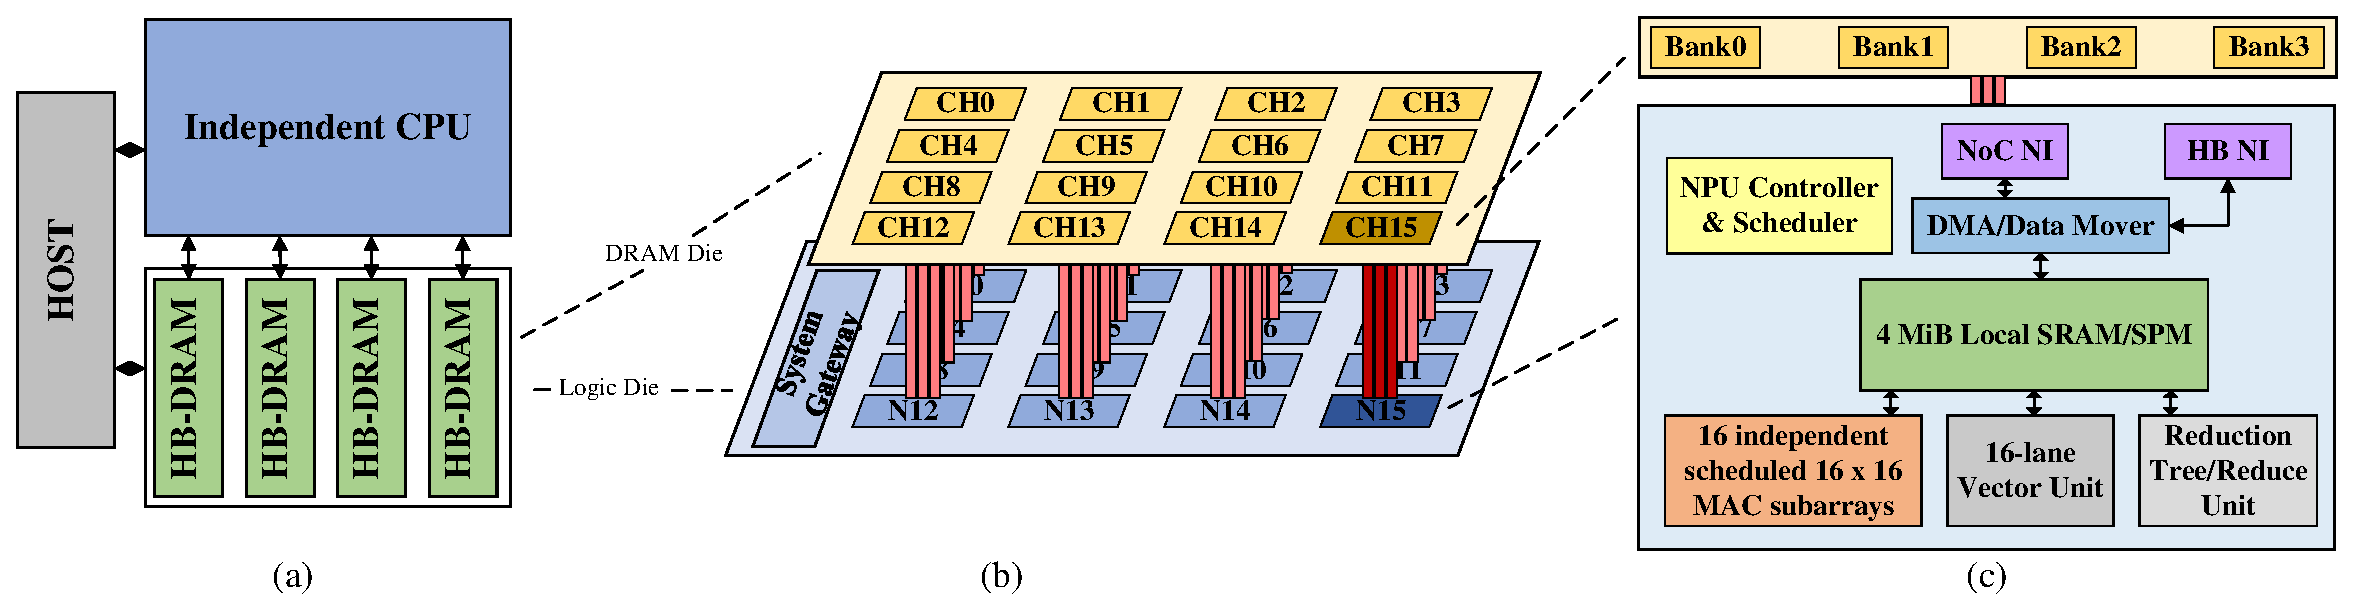
\includegraphics[width=\columnwidth]{figures/target_architecture.pdf}
  \caption{Target 3D system. (a) Host and HB-DRAM organization. (b) Face-to-face
  integration of the $4\times4$ Logic-tier NPU mesh and the aligned DRAM
  channels. (c) Microarchitecture of an NPU--memory pair.}
  \Description{Three panels show the host and HB-DRAM organization, the
  vertically aligned NPU clusters and DRAM channels, and the internal
  organization of one NPU--memory pair.}
  \label{fig:target-architecture}
\end{figure}

Figure~\ref{fig:target-architecture} shows a 3D accelerator in which the
logic and memory tiers are integrated by face-to-face hybrid bonding.
Each NPU cluster in the logic tier is vertically aligned with a DRAM
partition and accesses it through a local hybrid-bond link. A horizontal
$4\times4$ mesh NoC connects the NPU clusters and carries transfers between
them, including MoE dispatch and combine traffic. Local memory accesses and
inter-cluster transfers therefore use distinct physical paths. The vertical
alignment also couples the temperatures of the logic and DRAM tiers, so
concentrated activity in one tier can heat the other.

The main MoE evaluation covers Qwen3-30B-A3B~\cite{qwen3report} and
Qwen1.5-MoE-A2.7B~\cite{qwen15moe} for language-model inference,
mini-SWE-agent~\cite{minisweagent} with a Qwen3-30B-A3B backend for
SWE-bench Lite tasks~\cite{swebench}, and LingBot TI2V~\cite{lingbotvideo}
for video generation. The auxiliary thermal scenario combines
WHISPER~\cite{whisper}, an ORB-SLAM3-derived SLAM workload~\cite{orbslam3},
and $\pi_{0.5}$~\cite{pi05}.


\subsection{Phase-Dependent Congestion in MoE Communication}

\noindent\textbf{Problem.}
HiBand adapts communication locality by switching among four topologies---
Full-Local, Local-Biased, Global-Biased, and Full-Global---that repartition
bandwidth according to broad communication locality~\cite{wang2026hiband}.
MoE communication can concentrate transfers around a small set of busy NPU
nodes and links. When several messages need the same link or router output,
they must wait even if other parts of the network have spare capacity.
As hotspot locations change, the four predefined topologies may still leave
concentrated flows competing for the same links and router outputs, causing
persistent queueing despite spare capacity elsewhere.

Figure~\ref{fig:noc-phenomenon} shows the communication latency of
Qwen3-30B-A3B prefill. As input length increases
from 128 to 1024 tokens per request, the queueing share of mean network
round-trip latency rises from 57.2\% to 88.8\%, while mean zero-load latency
increases by 17.3\%. Zero-load latency includes serialization and traversal
without competing traffic; queueing is the additional delay under concurrent
traffic. Thus, queueing at shared network resources dominates the growth in
communication latency as input length increases.

\noindent\textbf{Root Cause.}
The gating network (Gate) selects a small set of experts for each token.
During Dispatch, token activations are sent to the NPU nodes holding those
experts; Combine returns the corresponding expert outputs. We define a flow
as the messages from one source NPU to one destination NPU within a single
communication phase. During Dispatch, when many tokens select the same experts, or several
frequently selected experts reside on the same NPU, transfers concentrate at
a small set of destinations. Flows whose routes overlap then compete for
shared links and router outputs, creating queueing hotspots. Thus, hotspot
formation depends on both the distribution of Gate selections and expert placement.
Our controlled Qwen3 decoding test also shows that concentrated accesses
can serialize requests at shared DRAM banks. Spreading those accesses across
banks addresses memory-side waiting, while overlapping NoC routes still
require path-level control.

Figure~\ref{fig:noc-cause} maps these messages onto deterministic XY paths.
Across MoE model layers 1, 24, and 48, the largest path-derived router demand
occurs at R9, R5, and R10, respectively. This spatial concentration can force multiple flows to share a
router output or link. Different concentrations can require different local
connections even when their total volume and aggregate communication locality
are similar. The design requirement is therefore to provide selectable local
paths around the contested resources, with explicit capacity at their
injection and receiving interfaces.

\begin{figure}[!tbp]
  \centering
  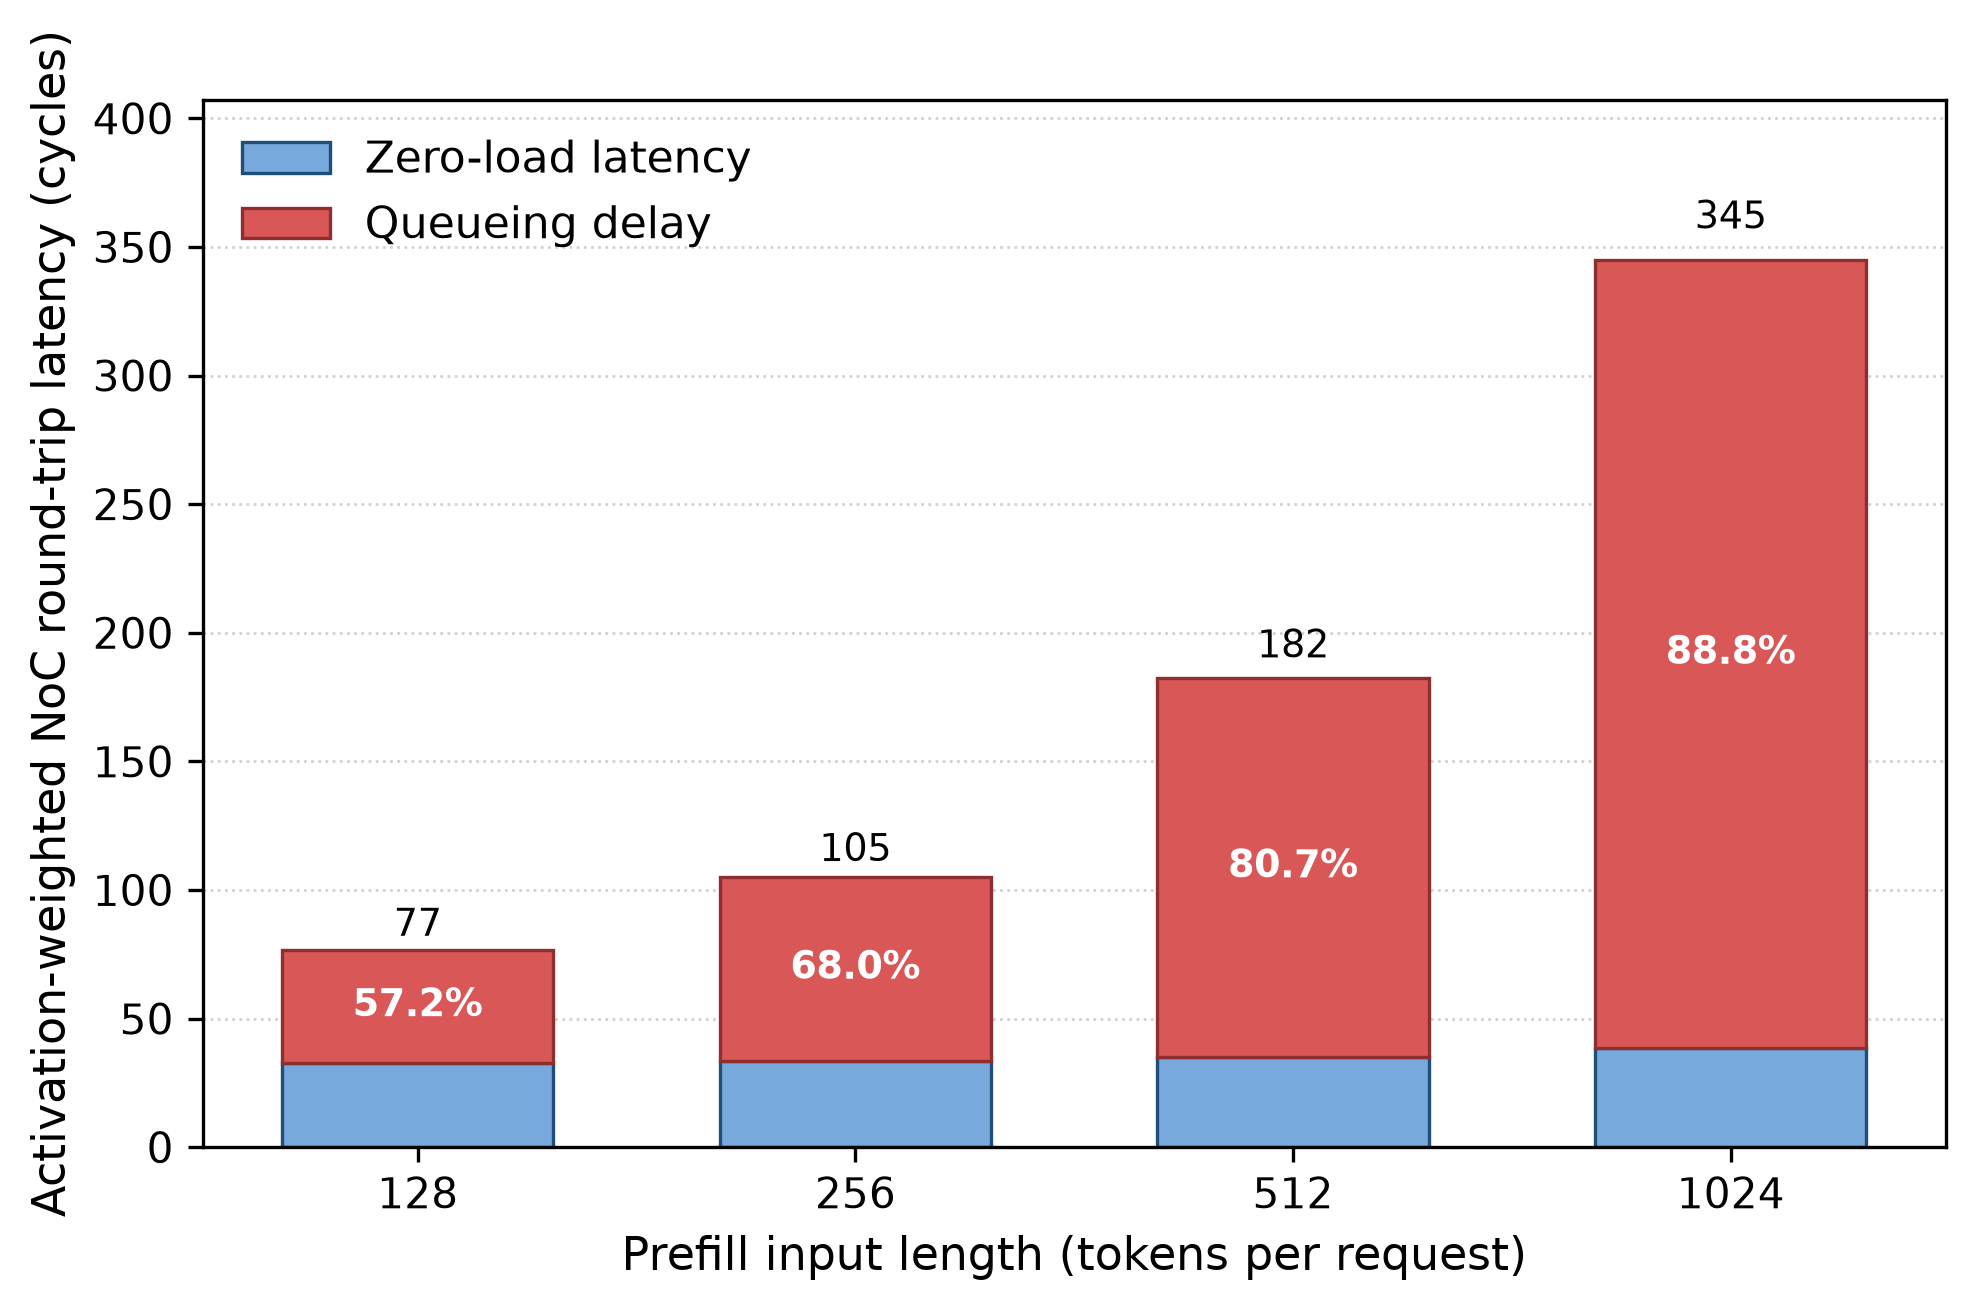
\includegraphics[width=\columnwidth]{figures/noc_phenomenon_input_tokens_0921.png}
  \caption{Qwen3-30B-A3B prefill communication on the fixed Mesh. Each bar
  reports the activation-weighted mean NoC round-trip latency at one input
  length. Zero-load
  latency contains serialization and uncongested traversal; queueing is the
  additional delay in the concurrent replay of the same message set. From 128
  to 1024 input tokens, the queueing share rises from 57.2\% to 88.8\%.}
  \Description{Four stacked bars for 128, 256, 512, and 1024 input tokens. The
  zero-load segment changes slightly, while the queueing segment grows rapidly
  and dominates the 1024-token bar.}
  \label{fig:noc-phenomenon}
\end{figure}

\begin{figure}[!tbp]
  \centering
  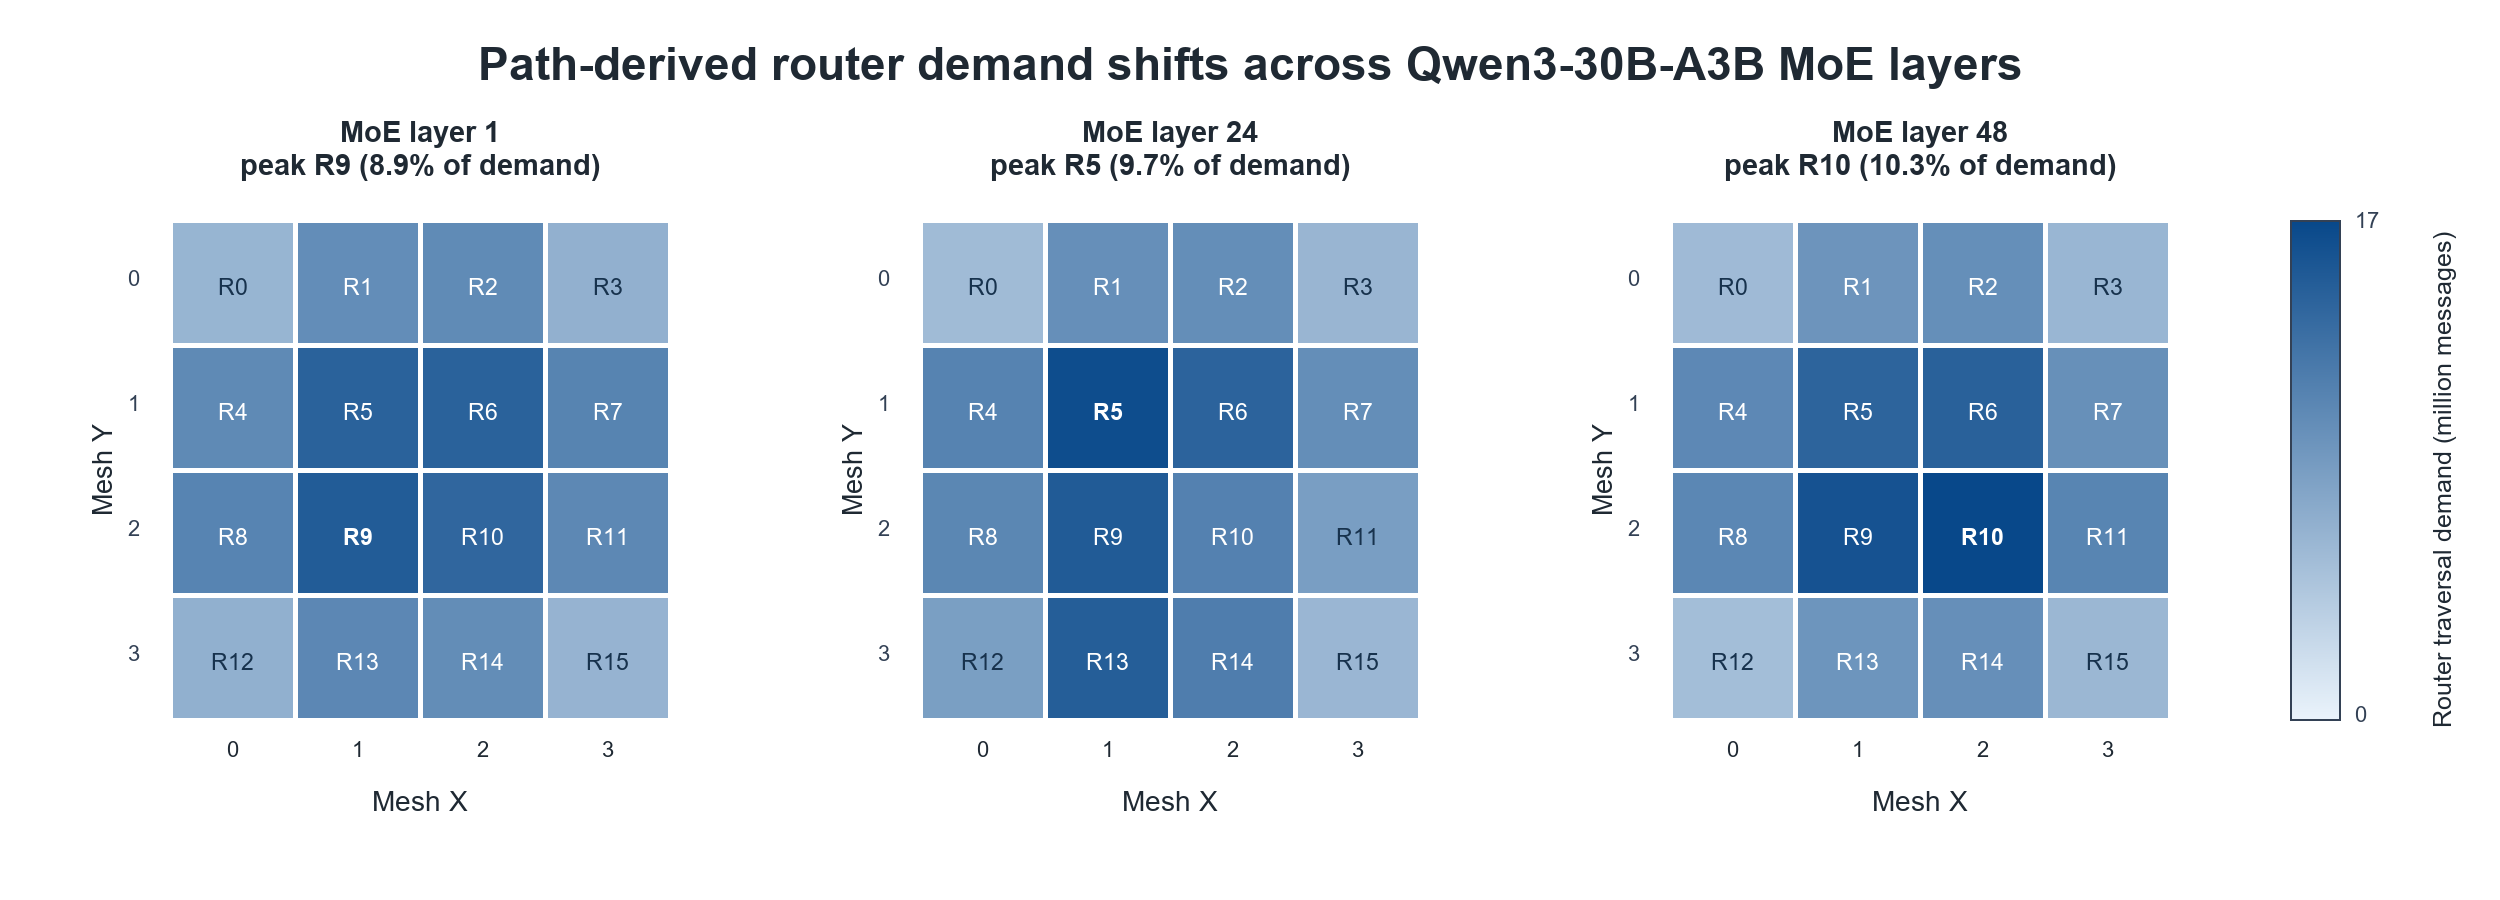
\includegraphics[width=\columnwidth]{figures/noc_cause_router_hotspots_revised.png}
  \caption{Path-derived router demand under the same Qwen3 trace. Each heatmap
  aggregates exact source--destination messages over every router on their
  deterministic XY path. With one shared scale, the peak moves
  R9$\rightarrow$R5$\rightarrow$R10 across
  MoE layers 1, 24, and 48, exposing a time-varying spatial demand pattern.}
  \Description{Three four-by-four router heatmaps for MoE layers 1, 24, and 48.
  The darkest cell changes location from router R9 to R5 and then R10.}
  \label{fig:noc-cause}
\end{figure}

\noindent\textbf{Opportunity: Configurable Local Connections.}
We place configurable switches (CSs) between neighboring NPU nodes in the same
Logic tier. Each switch selects connections between four fixed corner ports.
Using predicted hotspot locations, the controller configures nearby switches
to redirect selected transfers around congested links and router outputs,
and adjusts these connections as hotspot locations change. A selected
connection takes data from an auxiliary router output and delivers it directly
to the destination network interface (NI), bypassing intermediate Mesh routing
and the destination router's ordinary local output along that connection.
Traffic without a selected CS connection continues to use the Mesh.

Figure~\ref{fig:noc-opportunity} illustrates the mechanism. The XY route from
N2 to N5 traverses R2, R1, and R5. Switch C1 connects N1, N2, N5, and N6; setting
its northeast input to its southwest output permits the alternative
R2--C1--NI5 path. N2's transmit selector and N5's receive selector must both
select C1. This connection removes that transfer from the R1 path and R5 local
output and delivers the data to NI5's buffer-write interface.
When other messages compete for R1's output toward R5 or R5's local output,
diverting this transfer through C1 reduces the traffic using those outputs
and can relieve queueing.

\begin{figure}[!tbp]
  \centering
  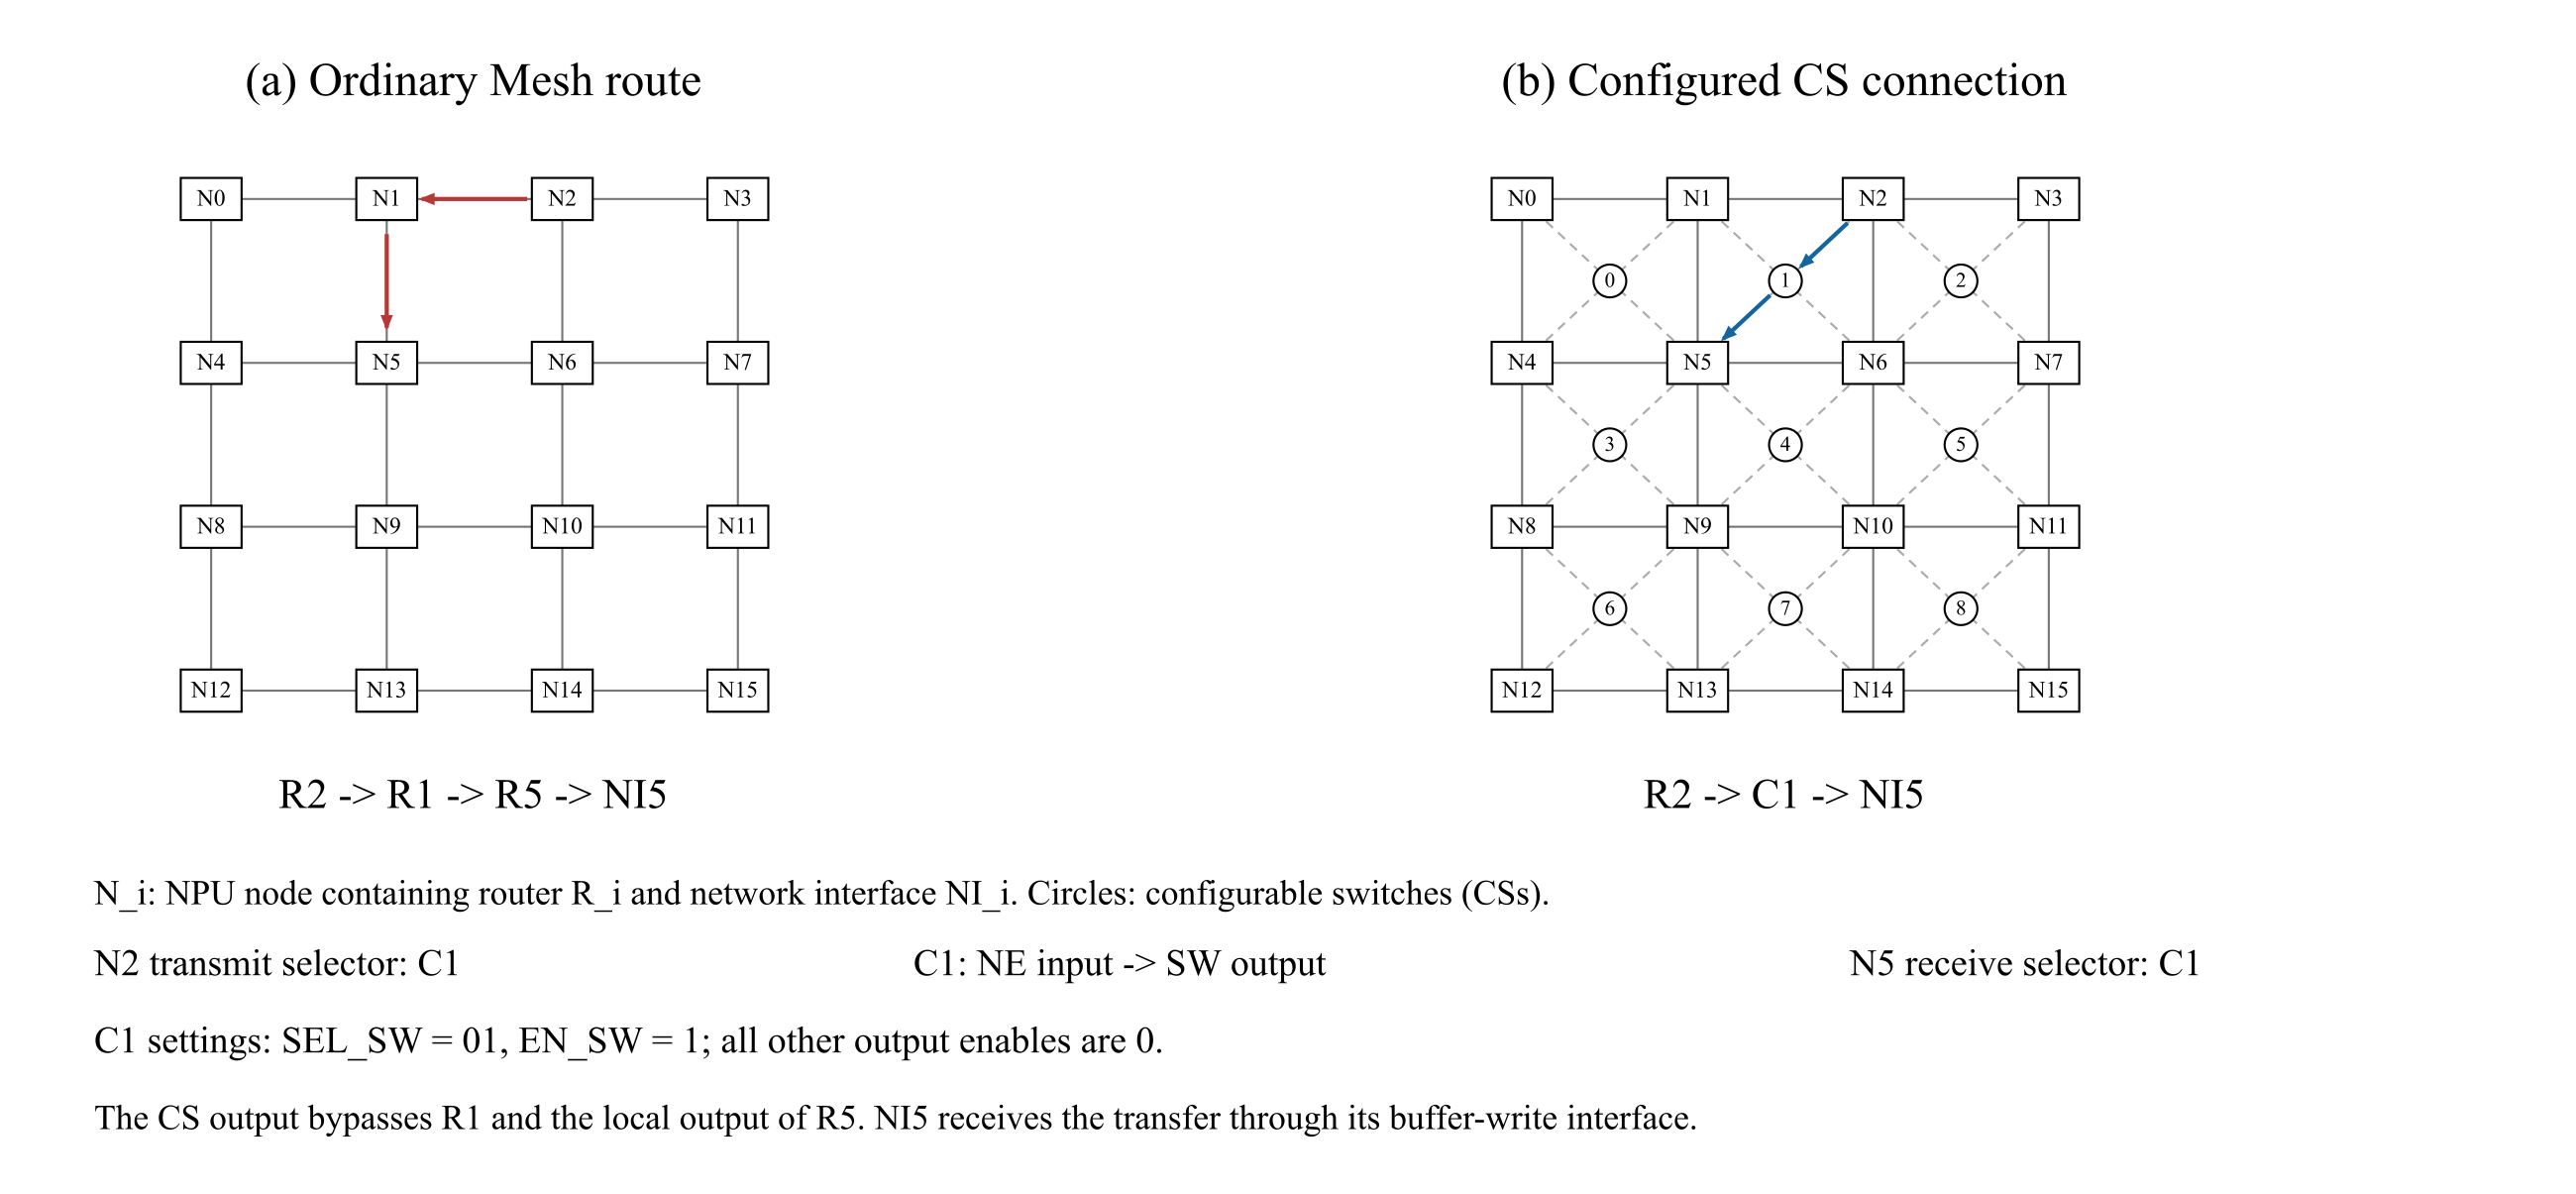
\includegraphics[width=\columnwidth]
  {figures/noc_opportunity_connection_example.png}
  \caption{Connection example for the NoC opportunity. (a) The ordinary
  N2-to-N5 route uses R1 and R5's local output. (b) A configured C1 connection
  delivers the transfer directly to NI5. The source transmit selector, CS
  connection, and destination receive selector are configured together.}
  \Description{Two four-by-four node layouts compare an ordinary Mesh route
  with a configured local-switch connection. A setting strip specifies N2 TX
  selection, the C1 northeast-to-southwest connection, and N5 RX selection.}
  \label{fig:noc-opportunity}
\end{figure}


Concentrating activity in a small region also affects the temperature of
both tiers. In our auxiliary thermal study, aligned logic and DRAM
hotspots persisted under AMBER-style thermal management~\cite{lin2026amber}.
This motivates using coupled temperature predictions to guide task
placement and regional DVFS.

\section{Design}
\label{sec:design}

\subsection{Reconfigurable Network}
\label{sec:noc-design}

Figure~\ref{fig:noc-physical-design}(a) shows the reconfigurable network
alongside the basic $4\times4$ Mesh. The logic tier contains sixteen NPU
nodes, nine lower-level configurable switches (CSs), and four upper-level
CSs. Nodes $N_0$--$N_{15}$ and lower CSs $\mathrm{CS}_0$--$\mathrm{CS}_8$
are indexed in row-major order. Each lower CS physically connects to
the NIs of the four corner nodes of a $2\times2$ group. A corner, edge, or interior node
therefore connects to one, two, or four lower CSs, respectively.
The upper CSs form a $2\times2$ network:
$\mathrm{CS}_9$, $\mathrm{CS}_{10}$, $\mathrm{CS}_{11}$, and
$\mathrm{CS}_{12}$ connect down to $\mathrm{CS}_0$, $\mathrm{CS}_2$,
$\mathrm{CS}_6$, and $\mathrm{CS}_8$, respectively.
Each upper CS connects to its corresponding lower CS and two upper
neighbors. For a local transfer, a lower CS selects one node-facing
input and a different node-facing output. A connection between a node
and the upper network instead selects one node-facing direction and U.
The upper network provides additional paths between the four lower
CSs attached to it. Upper CSs reach NPU nodes through these lower CSs.
The two CS levels are connectivity levels within the same logic die.
Their MUXes, configuration registers, and control gates are implemented
as logic cells, with the connections routed in the die's metal stack.
The separated planes in the figure depict this connectivity hierarchy.

Figure~\ref{fig:noc-physical-design}(b) shows the two CS circuits.
A lower CS has four corner directions, northwest (NW), northeast (NE),
southwest (SW), and southeast (SE), and an upper direction U.
Only the four lower CSs listed above have a physical U attachment.
In the other five instances, the U input data and valid signals are
tied to zero, the U output enable is hardwired to zero, and the
U-side ready input is tied to zero. These constant connections are
fixed at implementation time and cannot be changed by configuration
writes. Figure~\ref{fig:noc-physical-design}(b) depicts the lower-CS
circuit with a connected U direction. An upper CS has two in-plane
directions and a downward direction D. The lower and upper circuits
use five 4:1 multiplexers (MUXes) and three 2:1 MUXes, respectively.
Each output MUX is wired to the other directions' inputs, excluding
a return to its own direction. The configuration register supplies
an output-direction code, an input-selection code, and a connection
enable (EN). Direction decoding enables at most one output, so each
CS establishes at most one directed input--output connection.

A short transfer between two nodes attached to the same lower CS can
use that CS directly between its source and destination NIs.
This circuit provides an additional data channel alongside the Mesh,
increasing the available path bandwidth and moving part of the traffic
away from contended Mesh links and router outputs. Circuits through the
upper network connect nodes attached to different U-connected lower
CSs, bypassing intermediate Mesh routers.
Multiple CS attachments allow a node to participate in separate circuits.
A heavily communicating neighboring pair can use an additional CS path
alongside its Mesh connection. These connections can be reassigned as the
busy endpoints and node pairs change between communication phases.
Traffic without an assigned circuit uses the ordinary Mesh.
The aggregate transfer rate is also limited by NI service and SRAM
bank bandwidth.

\begin{figure*}[!t]
  \centering
  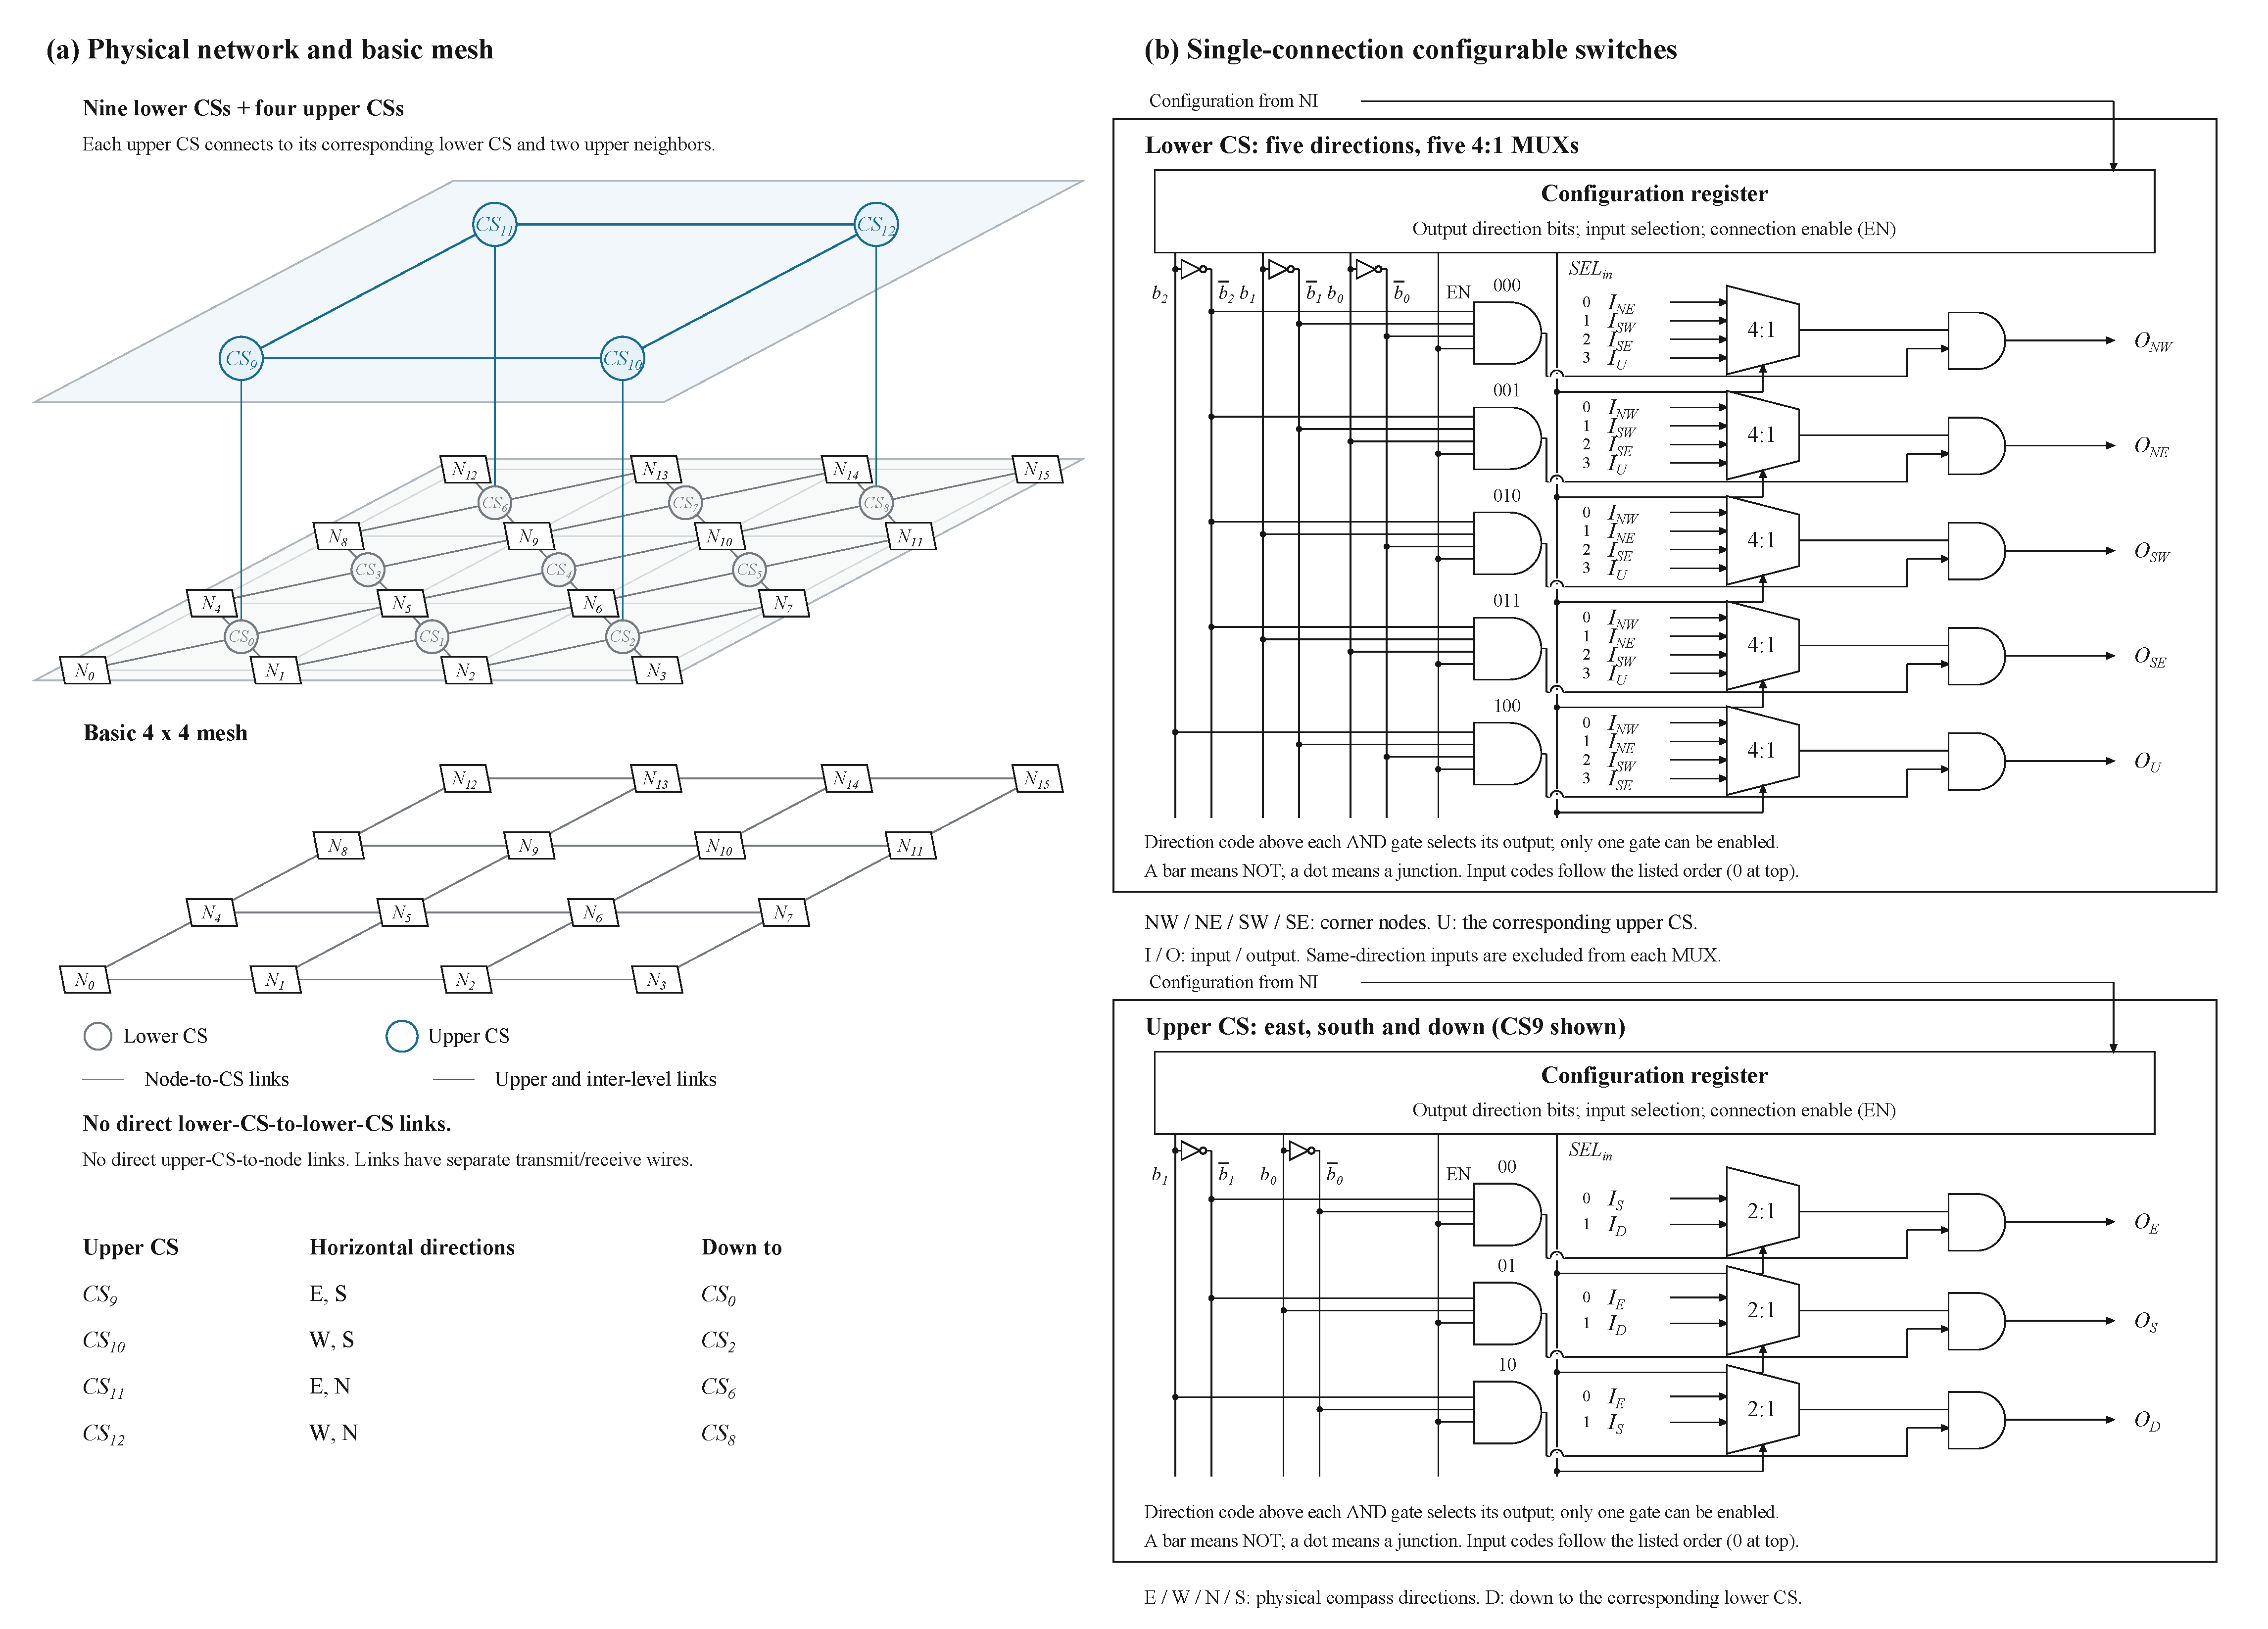
\includegraphics[width=\textwidth]{figures/noc_topology_cs.pdf}
  \caption{Reconfigurable network and switch circuits.
  (a) Nine lower CSs and four interconnected upper CSs, with the basic
  Mesh shown for comparison. The separated planes denote connectivity
  levels on one logic die. (b) A U-connected lower CS and an upper CS.
  Each MUX excludes its own direction's input; output decoding enables
  one connection.}
  \Description{The left panel shows the two levels of configurable switches
  and a basic Mesh. Only four lower switches attach to upper switches.
  The right panel expands the five-direction lower switch and
  three-direction upper switch, including configuration registers,
  direction decoding, input MUXes, and output enable gates.}
  \label{fig:noc-physical-design}
\end{figure*}

\subsection{Node and Network Interface}
\label{sec:noc-node-design}

Figure~\ref{fig:noc-node}(a) expands an NPU node. Its NPU cluster contains
a multiply--accumulate (MAC) array and a vector unit. A banked SRAM
scratchpad holds local weights and activations. The SRAM access controller
arbitrates bank requests from the NPU and the network interface (NI).
The Mesh router retains its four directional connections and a local
NI connection. The NI also has separate transmit and receive connections
to each adjacent lower CS. NW, NE, SW, and SE beneath the CSs in this
figure identify their positions relative to the node; a CS northwest
of the node uses its own SE direction to reach that node.

\begin{figure*}[!t]
  \centering
  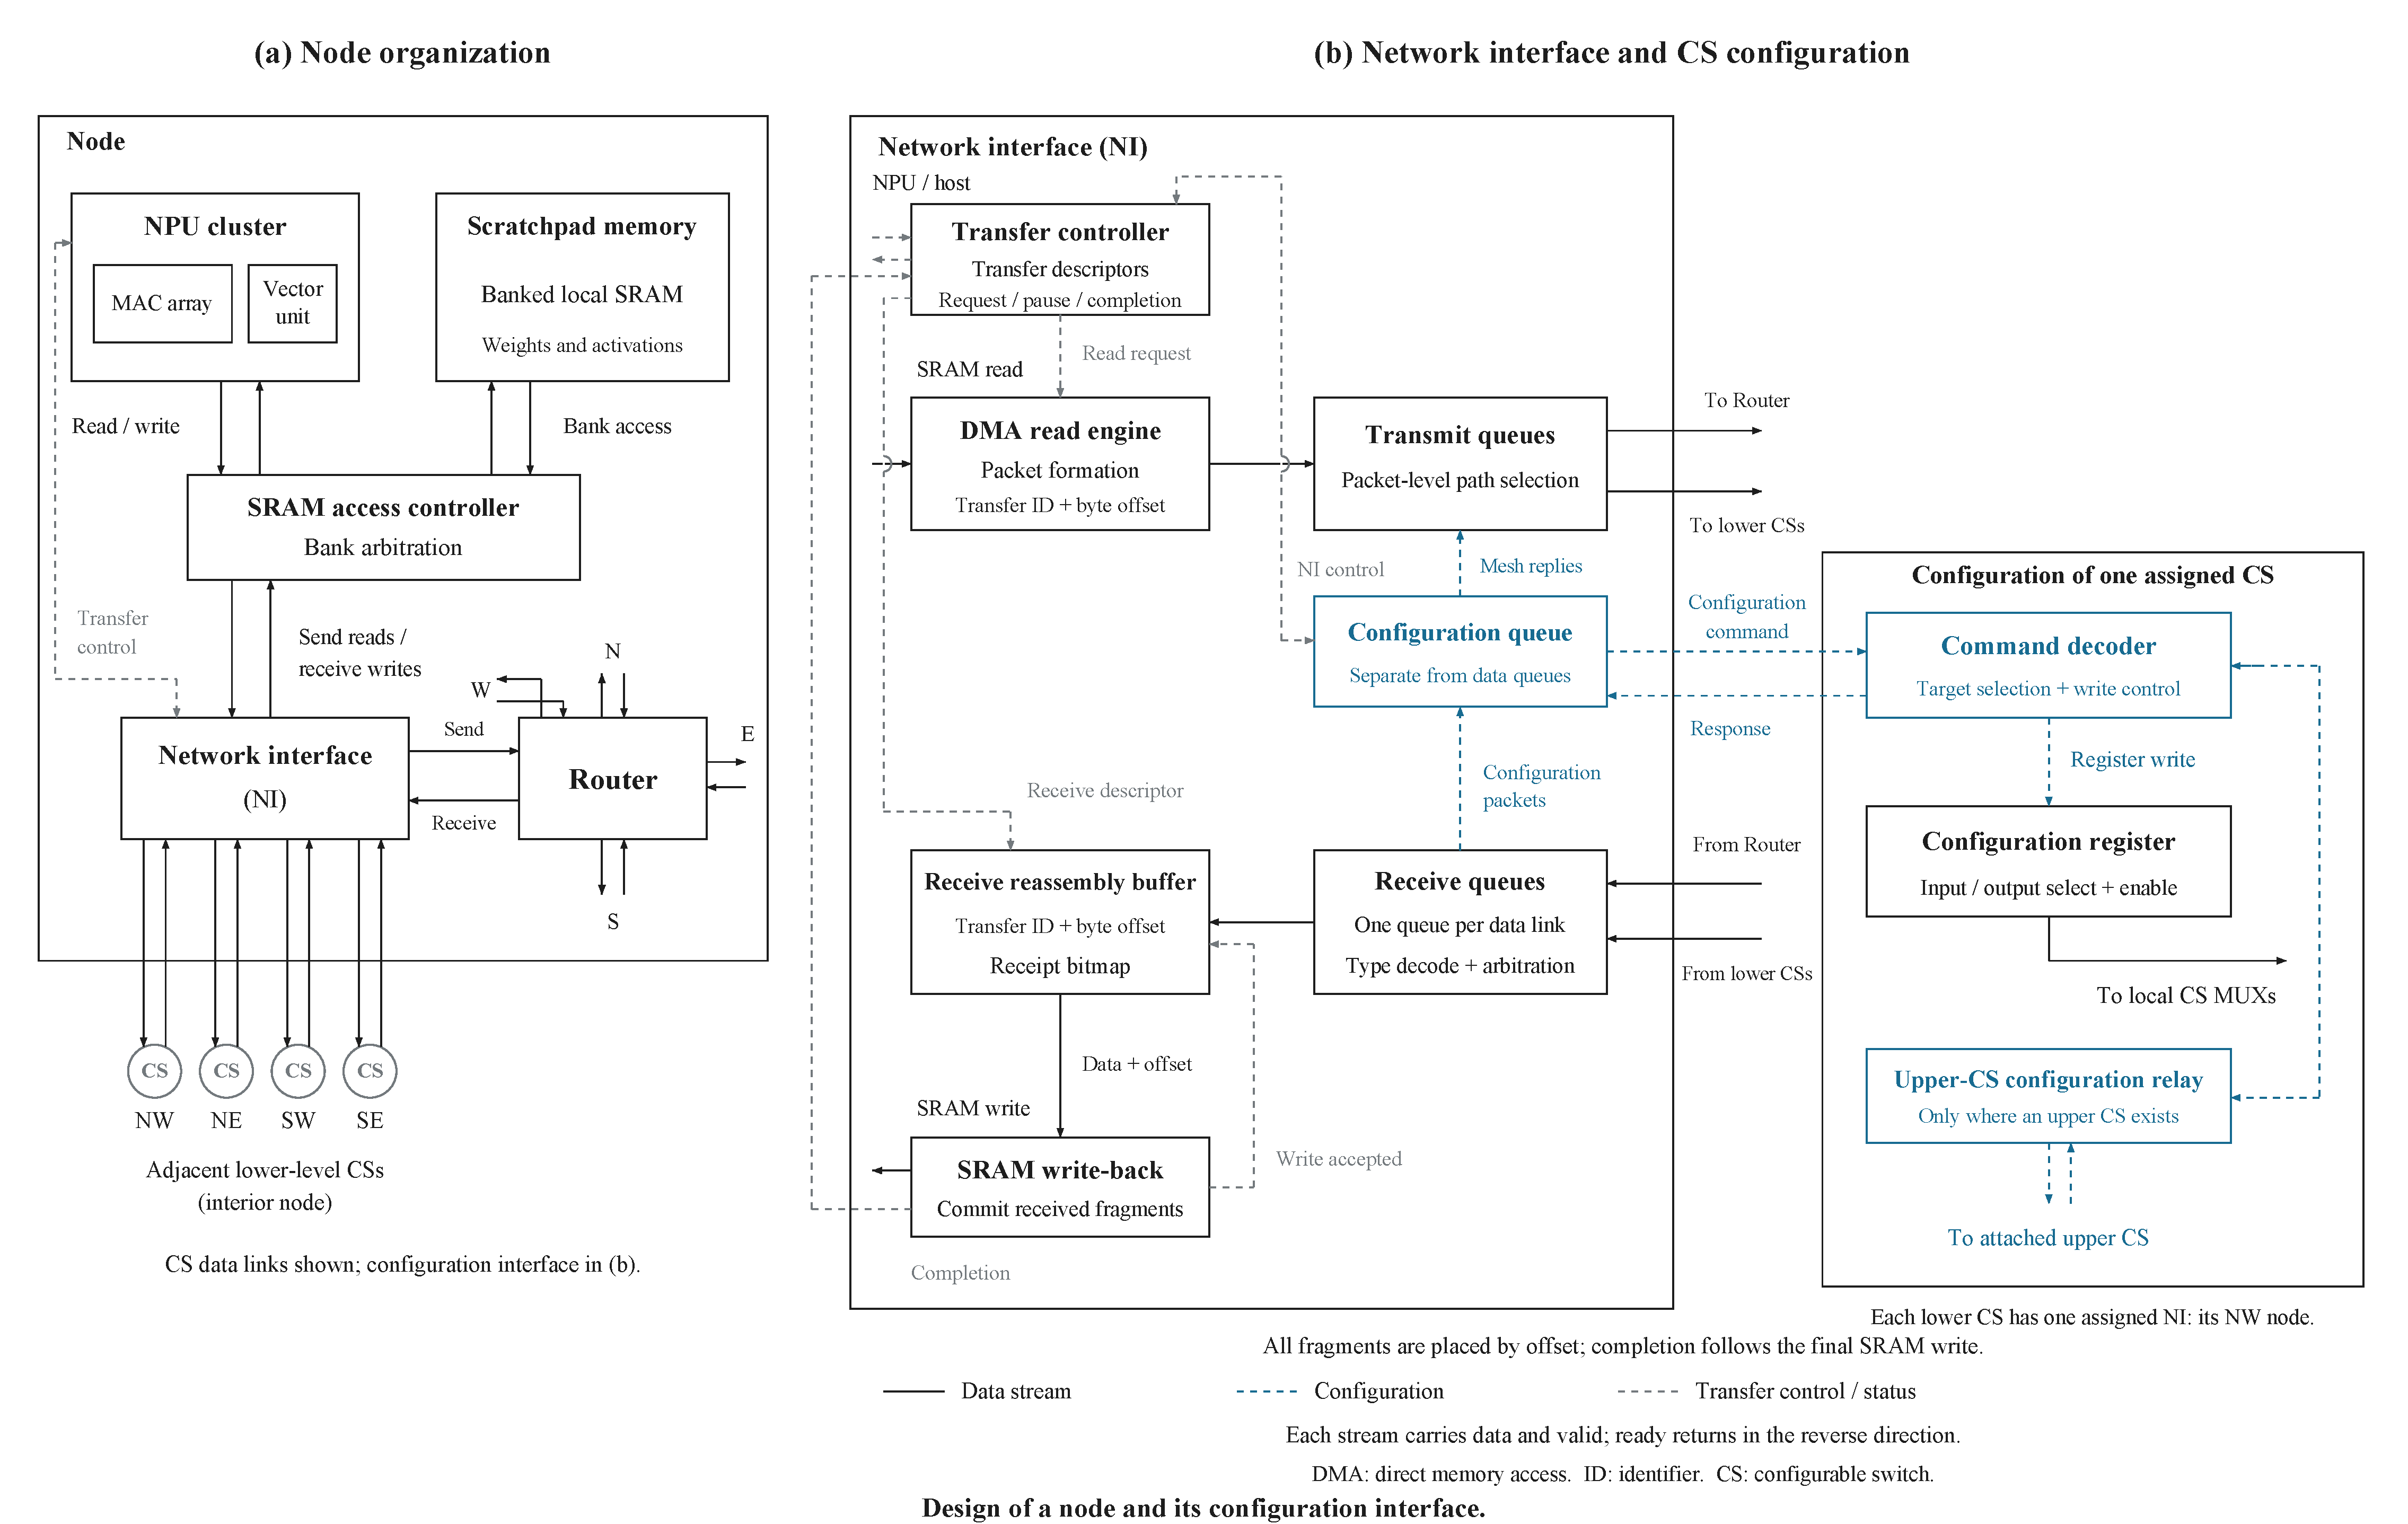
\includegraphics[width=\textwidth]{figures/noc_node_ni.pdf}
  \caption{Node and NI organization.
  (a) NPU, scratchpad, NI, Mesh router, and adjacent lower-CS data
  connections. (b) NI transmit, receive, and reassembly paths, together
  with the configuration interface of one assigned CS.
  Each lower CS is configured by its northwest node's NI.}
  \Description{A node contains an NPU cluster, local SRAM, shared bank
  arbitration, a network interface, and a Mesh router. The NI has separate
  adjacent-CS data streams. The expanded NI shows transfer control,
  packet formation, finite receive queues, offset-based reassembly,
  SRAM write-back, and a separate configuration queue. A CS-side decoder
  writes the configuration register and relays commands to an attached
  upper CS where present.}
  \label{fig:noc-node}
\end{figure*}

Figure~\ref{fig:noc-node}(b) shows the NI data path. The transfer controller
receives descriptors specifying the source and destination nodes, SRAM
addresses, and transfer length. A direct memory access (DMA) read engine
fetches source data and forms packets using the NI's configured payload
size. The final packet carries the remaining bytes. The sending and
receiving NIs use the same payload-size setting for a transfer.
Transmit queues select the Mesh or an assigned CS circuit for each complete packet.
A transfer may use several paths across its packets; the flits within
one packet follow the same path.
Each incoming data connection has a finite receive queue. Receive
arbitration feeds the reassembly buffer, while packet-type decoding
separates configuration commands from data.
CS streams carry data and a valid indication forward, with a ready
indication returning along the selected path. A transfer occurs when
valid and ready are both asserted.

Each data packet identifies its transfer by \texttt{TransferID}, formed
from the source NI and a source-local sequence number.
\texttt{Offset} gives its byte position within the transfer, and
\texttt{Length} gives the total transfer size. Receive descriptors
associate a transfer with its destination SRAM base address.
The NI derives each packet's index and expected payload length from
its offset, the transfer length, and the agreed payload size. It checks
the transfer identifier, offset alignment, and payload length before
writing the payload to the base address plus \texttt{Offset}.
A receipt bitmap has one bit per expected packet, updated after the
SRAM accepts that packet's payload write; already-received packets are
identified by their set bits. Transfers are admitted after allocating
their receive descriptors and bitmap storage.
Payloads can be written in arrival order while their offsets restore
the destination data layout.
The NI reports completion after all expected packet writes have completed;
the NPU then consumes the assembled data. This permits bounded
receive staging without holding later fragments until earlier ones
arrive. Reassembly writes and NPU accesses share the SRAM bank arbiter.

% TODO: Traffic prediction.
% \subsection{Traffic Prediction}
% \label{sec:traffic-prediction}

% TODO: Reconfiguration problem.
% \subsection{Reconfiguration Problem}
% \label{sec:noc-problem}

% TODO: Configuration algorithm.
% \subsection{Configuration Algorithm}
% \label{sec:noc-algorithm}

\subsection{Configuration Interface}
\label{sec:noc-config-interface}

The host CPU sends configuration packets over the ordinary Mesh to the
NI assigned to the target CS. Each lower CS is assigned to the NI of
its northwest corner node. This fixes one configuration writer per CS,
independently of its four neighboring data connections.
The NI places commands in a separate configuration queue and sends them
through a local command/response interface to the CS-side configurator.
The CS-side command decoder acts as the configurator: it decodes the
target and operation, writes the CS configuration register, and returns
a response.
For an upper CS, the corresponding lower CS relays the command and
response over a fixed inter-level control interface.
These local control interfaces operate independently of the CS data
MUX settings. Responses return through the NI and ordinary Mesh.

Table~\ref{tab:noc-command-fields} defines the packet and command fields.
A CS state is $q_c=(s_c^{\mathrm{out}},s_c^{\mathrm{in}},e_c)$, where
$c\in\{0,\ldots,12\}$ identifies the target CS,
$s_c^{\mathrm{out}}$ selects its output direction,
$s_c^{\mathrm{in}}$ selects an allowed input at that output's MUX,
and $e_c$ enables the connection.
The lower CS uses three output bits, two input bits, and one enable bit;
the upper CS uses two output bits, one input bit, and one enable bit.
Lower output codes 000--100 select NW, NE, SW, SE, and U, respectively.
Upper codes 00, 01, and 10 select the instance's horizontal direction,
vertical in-plane direction, and D. Input codes follow the remaining
input order shown at each MUX. A cleared enable or an unused output
code disables the connection.

\begin{table}[!t]
  \caption{Configuration packet and command fields.}
  \label{tab:noc-command-fields}
  \centering
  \small
  \begin{tabularx}{\columnwidth}{@{}p{0.25\columnwidth}>{\raggedright\arraybackslash}X@{}}
    \hline
    Field & Meaning \\
    \hline
    Type & Distinguishes configuration commands, responses, and data. \\
    Destination & Mesh destination NI assigned to the target. \\
    TransactionID & Matches a request to its response. \\
    Target & CS index $c$ for a register write. \\
    Operation & CS register write, or NI pause, status, and resume control. \\
    State & CS register tuple $q_c$ for a write. \\
    Status & Completion or failure reported in a response. \\
    \hline
  \end{tabularx}
\end{table}

The response echoes \texttt{TransactionID} and \texttt{Target};
an upper-CS write is acknowledged after the upper register accepts it.
The NI handles its own pause, status, and resume commands locally.
They control transfer admission and completion reporting, while
CS-targeted commands go to the CS-side configurator.

To change the network, the host first pauses admission of new CS
transfers at all NIs. Previously admitted transfers finish transmission,
reassembly, and SRAM write-back. The host collects their drain responses
over the Mesh, writes the new CS states, and waits for every target's
write response before resuming admission. A failed or incomplete update
keeps CS transmission paused. This sequence prevents data from
traversing a partially updated circuit.

% TODO: Brief thermal-management mechanism.
% \subsection{Thermal Management}
% \label{sec:thermal-management}

\FloatBarrier

\section{Evaluation Results and Analysis}
\label{sec:experiment}

\subsection{Experimental Setup}

We evaluate the proposed design on a face-to-face hybrid-bonded 3D accelerator. Table~\ref{tab:eval-platform} lists the common platform parameters. The evaluation uses 32~GiB of HB-DRAM. Each comparison starts from the same input and initial system state and uses the same precision, resource budget, and workload completion criteria. We account for each method's additional hardware and runtime costs separately.

\begin{table}[t]
\caption{Common hardware and simulation settings.}
\label{tab:eval-platform}
\centering\small
\begin{tabular}{@{}lp{0.59\columnwidth}@{}}
\hline
Component & Configuration \\
\hline
Logic tier & 16 NPU clusters at 1~GHz \\
NPU cluster & 4096 MACs, 16-lane vector unit, 4~MiB SRAM \\
Base NoC & $4\times4$ mesh, 256-bit links at 1~GHz \\
HB-DRAM & 32~GiB, 16 partitions of 2~GiB each, 16 logical banks per partition \\
Vertical link & 25.6~GB/s per NPU--memory pair \\
Host & Four CPU cores, PCIe 5.0, host memory xxx \\
Simulation & Compute, memory, and NoC models xxx \\
Thermal model & Ambient and initial temperatures xxx, temperature limit xxx \\
\hline
\end{tabular}
\end{table}

Table~\ref{tab:eval-workloads} lists four main MoE workloads and one auxiliary thermal scenario. We freeze the input manifests, arrival order, seeds, and stopping rules before collecting performance results.

\begin{table*}[t]
\caption{Workloads, input manifests, and measurement boundaries.}
\label{tab:eval-workloads}
\centering\small
\begin{tabularx}{\textwidth}{@{}p{0.25\textwidth}Xp{0.29\textwidth}@{}}
\hline
Workload & Inputs and configuration & Measurement boundary \\
\hline
Qwen3-30B-A3B & Prompt source and IDs xxx, input/output lengths xxx, concurrency xxx & Prefill, decode, and complete request \\
Qwen1.5-MoE-A2.7B & Prompt source and IDs xxx, lengths xxx, TP/PP mapping xxx & Prefill, decode, and complete request \\
mini-SWE-agent + Qwen3 & SWE-bench Lite instance IDs and split xxx, tool and stopping rules xxx & Model calls, full agent task, and task outcome \\
LingBot TI2V & Text/image IDs xxx, resolution xxx, frames xxx, steps and seeds xxx & Encoding, denoising, scheduler, and VAE decoding \\
WHISPER + SLAM + $\pi_{0.5}$ & WHISPER version xxx, SLAM and $\pi_{0.5}$ traces xxx, request schedule xxx & Joint thermal scenario, execution coverage xxx \\
\hline
\end{tabularx}
\end{table*}

For each experimental line, we first run the complete workload under both configurations and record stage latencies and the end-to-end critical path. Subsequent paired points measure the same one or two MoE layers with identical input and routing samples. We extrapolate both arms using the same layer selection, weights, and dependency model, including non-MoE stages and control costs. Recomputing the critical path preserves overlap among compute, memory, and communication. We validate the estimates against the complete runs and report measured layer latency, estimated end-to-end latency, and estimated speedup separately. The corresponding estimation errors are xxx. All reported execution times refer to the modeled target system.

\subsection{End-to-End Performance Comparison}

The primary comparison pairs the common platform baseline B with B plus the full design. We separately compare with prior methods that pass the same workload and timing checks under matched resource constraints. The HiBand reference implementation and other candidate NoCs enter this comparison after qualification. Table~\ref{tab:eval-comparisons} records the scope of each comparison.

\begin{table}[t]
\caption{Configurations and scope of the performance comparisons.}
\label{tab:eval-comparisons}
\centering\small
\begin{tabular}{@{}lp{0.53\columnwidth}@{}}
\hline
Configuration & Comparison scope \\
\hline
B & Common platform baseline, frozen configuration xxx \\
B + full design & Paired end-to-end comparison with B \\
HiBand reference & External comparison, qualification pending \\
Other NoC candidates & Configurations and qualification results xxx \\
\hline
\end{tabular}
\end{table}

Figure~\ref{fig:eval-overall} compares completion times for each main workload. For each pair, we compute the latency reduction as $1-T_{\mathrm{design}}/T_{\mathrm{ref}}$, where $T_{\mathrm{ref}}$ is the completion time of B or the named external comparator. We also report time to first token and time per output token for the language-model workloads. For mini-SWE-agent, we report model-call latency and task latency separately and record task outcomes. For LingBot, we report the latency of a complete generation. The measured end-to-end latencies, paired reductions, and workload-level exceptions are xxx.

\begin{figure*}[t]
\centering
\fbox{\rule{0pt}{18mm}\rule{0.92\textwidth}{0pt}}
\caption{End-to-end latency by workload for B, B plus the full design, and qualified external comparators. Each panel uses identical inputs and completion criteria. Labels distinguish complete-run measurements from estimates based on sampled MoE layers.}
\Description{Reserved space for the end-to-end latency comparison.}
\label{fig:eval-overall}
\end{figure*}

\subsection{Supporting Results and Thermal Ablation}

\paragraph{Phase-dependent congestion and bank waiting.}
To explain the latency differences in Figure~\ref{fig:eval-overall}, we trace matched MoE communication phases from memory requests through consumer readiness. We measure bank queueing before data becomes available, injection and router queueing, unloaded traversal, and synchronization at the slowest endpoint. We record configuration delay on the same timeline and attribute only exposed delays to the critical path. Comparing packet tails and router activity across phases tests whether a change in hotspot location translates into earlier consumer readiness. A comparison with fixed network policy and a bank-policy toggle can isolate the incremental effect of bank conflict mitigation. The paired changes in exposed waiting and packet tail latency are xxx.

\begin{figure*}[t]
\centering
\fbox{\rule{0pt}{17mm}\rule{0.92\textwidth}{0pt}}
\caption{Critical-path latency breakdown for matched MoE communication phases. The timeline shows bank service, data readiness, NoC injection and queueing, configuration, and consumer synchronization. Companion panels show packet tail latency and router activity using common scales across configurations.}
\Description{Reserved space for the critical-path breakdown and congestion panels.}
\label{fig:eval-breakdown}
\end{figure*}

\paragraph{Incremental effect of thermal management.}
We compare NoC with bank conflict mitigation and thermal management against the same NoC and bank mechanisms with thermal management disabled. Both arms start with identical temperatures, inputs, and thermal constraints. We track temperatures over the complete execution timeline and account for prediction, throttling, redistribution, and recovery where they occur. We report natural and thermally stressed scenarios separately. Peak temperature, time above the threshold, and completion time are xxx.

\begin{figure}[t]
\centering
\fbox{\rule{0pt}{17mm}\rule{0.90\columnwidth}{0pt}}
\caption{Temperature and workload progress with thermal management enabled and disabled. Both configurations use the same NoC and bank policies. Markers denote thermal triggers, throttling, and work redistribution where observed.}
\Description{Reserved space for temperature and workload progress curves.}
\label{fig:eval-thermal}
\end{figure}

\subsection{Scalability and Sensitivity Analysis}

We vary system scale and input scale separately. The system-scale sweep starts at 16 NPU clusters and holds workload fixed. At each scale, we report the topology, mapping, capacity, and bandwidth. The input-scale sweep fixes the platform and varies request concurrency or input size. We report absolute completion time and paired latency reduction at each point. To examine design sensitivity, we vary the local connection budget and reconfiguration interval one at a time and record completion time, packet tail latency, and exposed configuration cost. The tested ranges and observed trends are xxx.

\begin{figure}[t]
\centering
\fbox{\rule{0pt}{17mm}\rule{0.90\columnwidth}{0pt}}
\caption{Scalability and sensitivity. Panels show (a) system scale at fixed workload, (b) input scale at fixed system size, and (c) sensitivity to the local connection budget and reconfiguration interval. Markers indicate the default configuration and whether overall latency is measured or estimated.}
\Description{Reserved space for the scalability and parameter sweeps.}
\label{fig:eval-scale}
\end{figure}

\subsection{Hardware Cost and Runtime Overhead}

We report implementation costs for local switches, links and configuration logic, bank control, and thermal control. Table~\ref{tab:eval-cost} separates FPGA resource utilization, ASIC synthesis, and post-route results. Within each stage, baseline and enhanced implementations use the same tools and constraints. We state whether memories, physical interfaces, and cross-tier wiring are included and report module-level costs and system-level increments where available.

\begin{table}[t]
\caption{Hardware implementation cost by evaluation stage.}
\label{tab:eval-cost}
\centering\small
\begin{tabular}{@{}lp{0.63\columnwidth}@{}}
\hline
Stage & Conditions and reported results \\
\hline
FPGA prototype & Device/tool/clock xxx, LUT/FF/BRAM/DSP xxx, achieved frequency xxx \\
ASIC synthesis & Process/library/PVT/clock xxx, area xxx, power estimate xxx \\
Post-route ASIC & Extraction/PVT/activity xxx, area xxx, timing slack xxx, dynamic and leakage power xxx \\
\hline
\end{tabular}
\end{table}

Table~\ref{tab:eval-runtime} reports algorithm execution separately from the delay of applying its decisions. For each algorithm, we measure per-call time and call count, then report the fraction of total application latency exposed on the critical path. Configuration transfer, hardware reconfiguration, and thermal migration are accounted for as separate events.

\begin{table}[t]
\caption{Runtime overhead of online decision algorithms.}
\label{tab:eval-runtime}
\centering\small
\begin{tabular}{@{}lccc@{}}
\hline
Algorithm & Time/call & Calls & Exposed share \\
\hline
Hotspot prediction & xxx & xxx & xxx \\
Connection selection & xxx & xxx & xxx \\
Bank policy & xxx & xxx & xxx \\
Thermal control & xxx & xxx & xxx \\
\hline
\end{tabular}
\end{table}

\section{Related Works}
\label{sec:related-works}

\section{Conclusion}
\label{sec:conclusion}

\bibliographystyle{IEEEtran}
\bibliography{references,thermal_references}

\end{document}

